\copyrightVincent

\begin{frame}[fragile]{Tabellen}
    \begin{columns}
        \begin{column}{0.5\textwidth}
            \begin{minted}[fontsize=\scriptsize,escapeinside=~~]{tex}
                \usepackage{booktabs}
                \usepackage{tabularx}
                ...

                \begin{table}[htbp]
                    \centering
                    \begin{tabularx}{\textwidth}
                        {X>{\raggedleft\arraybackslash}X}
                        \toprule
                        Formule & Beschrijving\\
                        \midrule
                        $ \sqrt{2} $ & Wortel\\
                        $ \frac{2}{3} $ & Breuk\\
                        $ 6\geq 3 $ & Symbool\\
                        $ a^2 + b^2 $ & Superscript\\
                        \bottomrule
                    \end{tabularx}
                    \caption{Een tabel!}
                \end{table}
            \end{minted}
        \end{column}
        \begin{column}{0.5\textwidth}
            \begin{adjustbox}{frame=1pt 10pt}%
                \begin{minipage}{\textwidth-22pt}
                    \begin{table}[H]
                        \centering
                        \begin{tabularx}{\textwidth}{X>{\raggedleft\arraybackslash}X}
                            \toprule
                            Formule & Beschrijving\\
                            \midrule
                            $ \sqrt{2} $ & Wortel\\
                            $ \frac{2}{3} $ & Breuk\\
                            $ 6\geq 3 $ & Symbool\\
                            $ a^2 + b^2 $ & Superscript\\
                            \bottomrule
                        \end{tabularx}
                        \caption{Een tabel!}
                    \end{table}
                    \vspace{-20pt}
                \end{minipage}
            \end{adjustbox}
            % \adjustbox{bgcolor=white}{%
            %     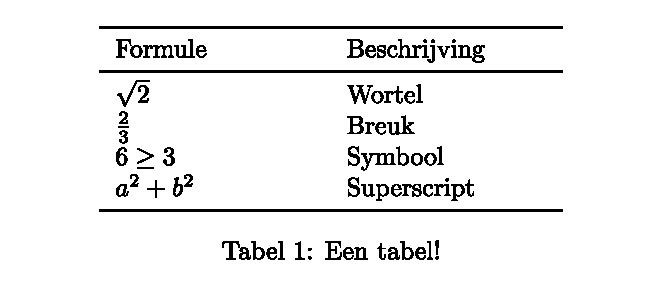
\includegraphics[width=\textwidth]{assets/tabellen1.pdf}%
            % }
        \end{column}
    \end{columns}
\end{frame}


